\chapter{Instalace a údržba}

\vspace{10pt}

Aplikace lze provozovat jako 2 oddělené celky, kterým můžeme říkat frontend a backend.

\vspace{10pt}

\textbf{Frontend}

Je rozhraní mezi aplikací a uživatelem, v tomto případě tedy webová aplikace běžící na Apache serveru s PHP modulem. Na stejném serveru může běžet i databáze.

\vspace{10pt}

\textbf{Backend}

Je ta část aplikace, která běží na pozadí a zajišťuje vlastní vyhotovování nahrávek. Ze serveru, kde běží backend, se také poté distribují výsledky. Pokud bychom neměli dostatek místa, je možná aplikaci dále rozdělit na další server, který by se staral o distribuci a nahrávky by se po uložení ukládaly na distribuční server třeba pomocí NFS sdílení. Naopak pokud budeme chtít může běžet backend na stejném serveru jako frontend.

\vspace{10pt}

\begin{figure}[ht]
\begin{center}
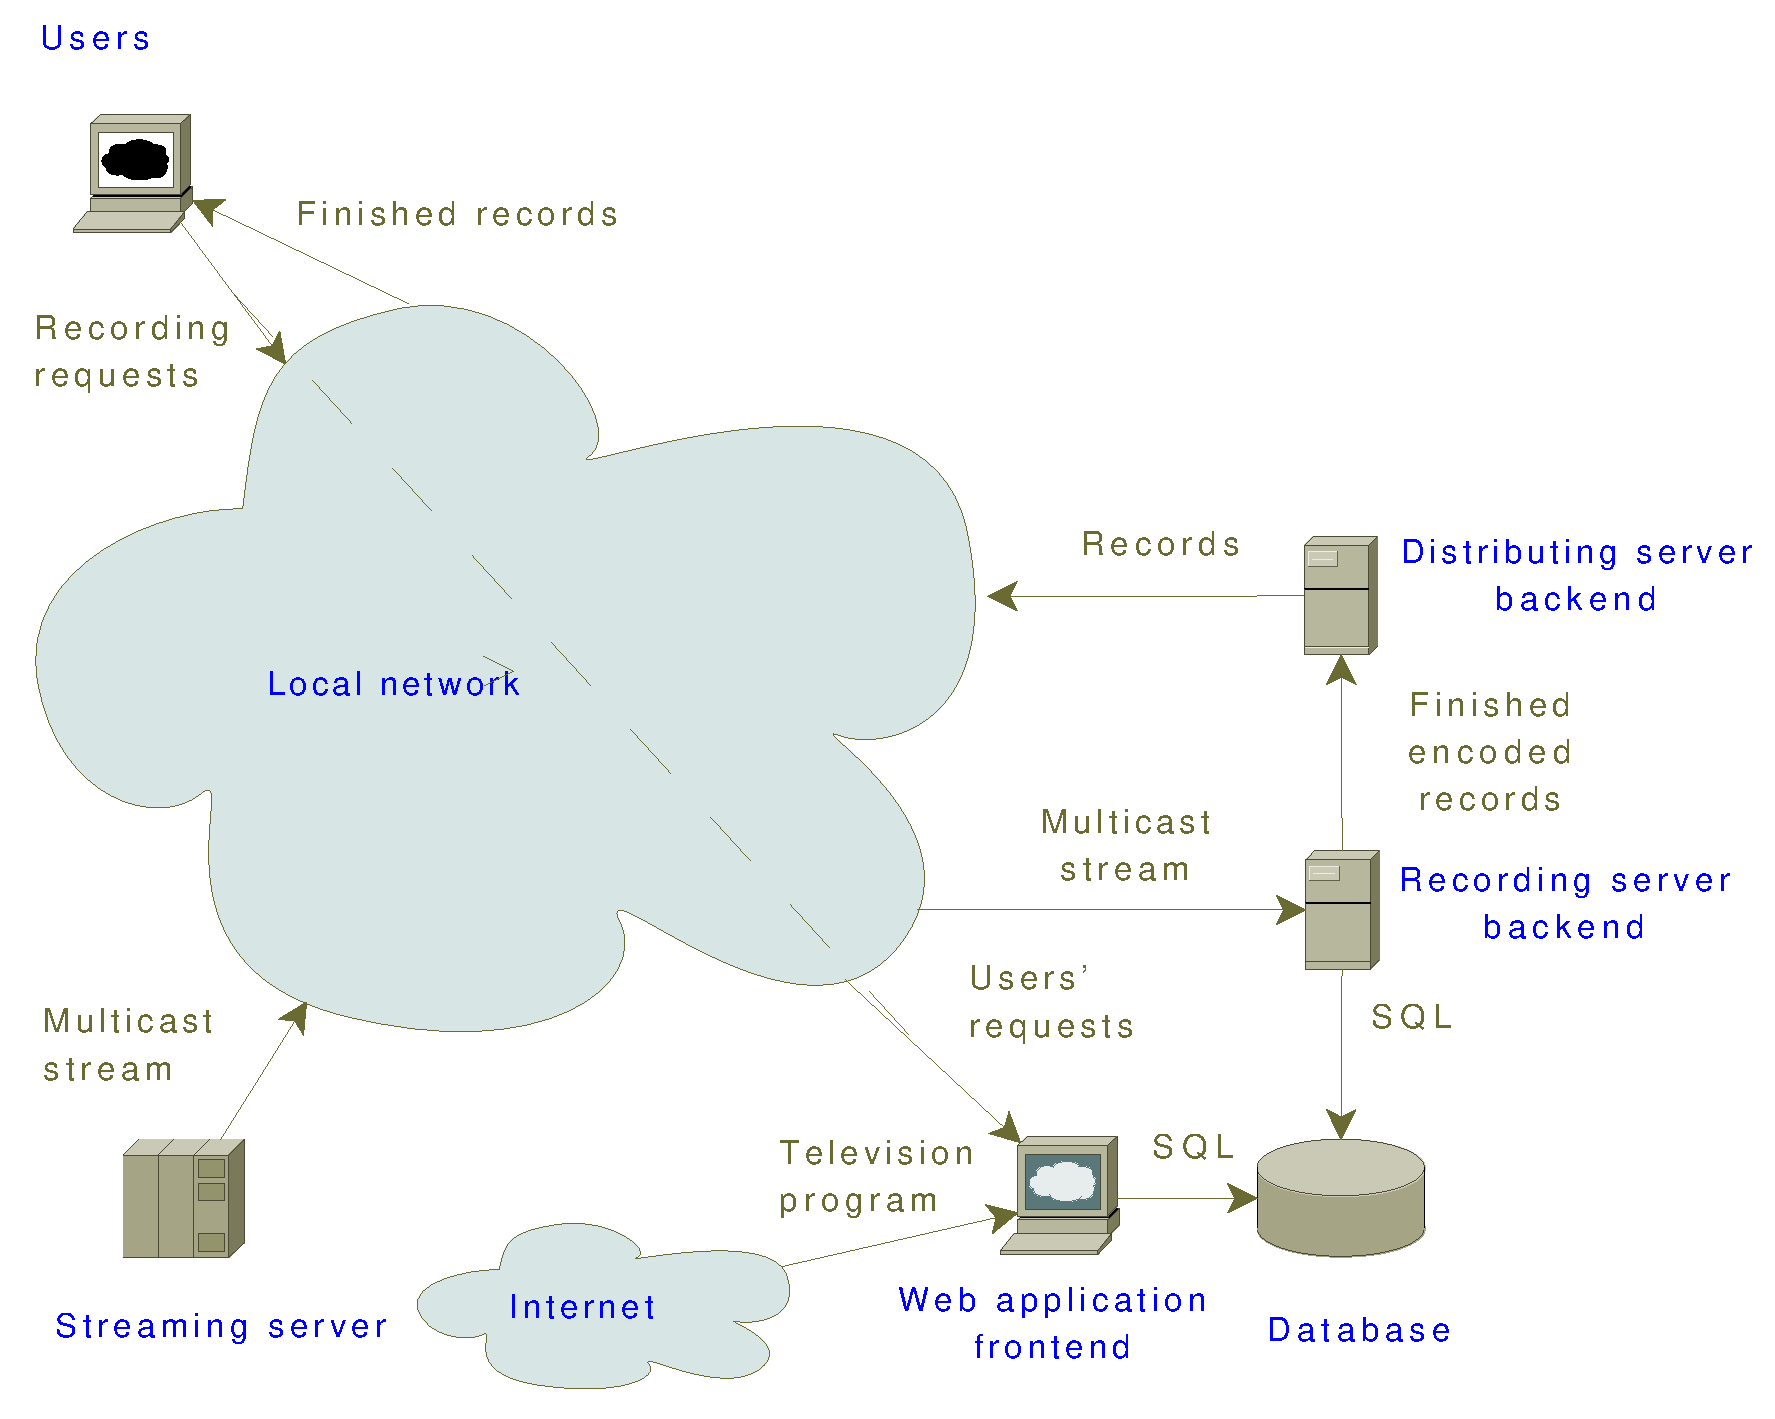
\includegraphics[width=15cm]{images/dvbgrab.eps}
\caption{Komponenty DVBgrabu}
\label{fig:dvbgrab}
\end{center}
\end{figure}

\section{Potřebné knihovny a pomocné programy}

\vspace{10pt}

\textbf{Apache}

Apache jako webový server budeme potřebovat jak na backend tak na frontend serveru.
Minimálně pro backend server je dobré použít buď verzi 1.x nebo až 2.2, protože verze 2.0 měla problémy se soubory většími nez 2GB, které jako graby často vznikají.

\vspace{10pt}

\textbf{PHP}

Na webovém serveru je potřeba modul do apache. Na záznamovém stačí PHP interpretr přístupný z příkazového řádku. Obvykle instalace stejně obsahuje oba. Aplikace byla otestována jak na PHP verze 4 tak 5, v PHP musí být povoleny některé rozšíření viz. dále.

\vspace{10pt}

\textbf{php-pear-Log}

Logovací systém, obdoba log4j pro Javu. Je potřeba na obou serverech a přes něj jsou zapisovány veškeré záznamy do logovacích souborů. Logovací soubory se používají 4 jsou v podadresáři log.

dvbgrab.log - obecné hlášky systému.

dvbgrab.log.sql - veškerý SQL kód, který je volán.

dvbgrab.log.sys - veškeré příkazy operačního systému, které jsou volány z PHP.

dvbgrab.log.clean - logování výstupu z údržbového skriptu.

Logování SQL a systémových příkazů může generovat poměrně velké logy, proto by mělo být po odladění aplikace vypnuto v dolib.inc.php.

\vspace{10pt}

\textbf{php-json}

Podpora pro JSON (JavaScript Object Notation) do PHP. JSON je použit pro dotazy na detail televizního pořadu nebo grabu v seznamu grabů. Je to alternativní notace která je vrácena na volání XMLHttpRequestu z javascriptu. Toto rozšíření usnadňuje generování JSON odpovědi ve skriptu, který z databáze detail načítá a zpracování přijaté odpovědi ve webové stránce.

\vspace{10pt}

\textbf{php-adodb}

Knihovna pro abstraktní přístup k různým databázím. Všechna volání do databáze překládá ze své syntaxe do syntaxe použitého databázového stroje.

\vspace{10pt}

\textbf{XMLTV}
Pokud chcete použít XMLTV modul pro načítání televizního programu bude potřeba nainstalovat tento balík. Buď v něm přímo najdete stahovací skript pro požadované programy, nebo se bude hodit alespon skript tv\_sort.

\vspace{10pt}

\textbf{Databáze}

DVBgrab by měl fungovat s libovolnou databází, která je podporována v adodb. Otestovaný je na postgresql a mysql, také skripty pro založení databáze jsou připraveny v syntaxy pro mysql a postgresql.

\vspace{10pt}

\section{Stažení DVBgrabu}

\vspace{10pt}

DVBgrab je dostupný na na sourceforge.net. K dispozici jsou jak jednotlivé uveřejněné verze, tak čtení z vývojového repozitáře subversion.

Odkaz na jednotlivé verze naleznete na stránkách projektu http://dvbgrab.sourceforge.net/.

Pro export vývojového repozitáře použijte následující:

\vspace{10pt}

Starší verze \textbf{dvbgrab-1.0}
\begin{small}\begin{verbatim}
svn export --username anonymous \
https://dvbgrab.svn.sourceforge.net/svnroot/dvbgrab/tags/dvbgrab-1.0 dvbgrab
\end{verbatim}\end{small}
Aktuální verze \textbf{dvbgrab-2.0}
\begin{small}\begin{verbatim}
svn export --username anonymous \
https://dvbgrab.svn.sourceforge.net/svnroot/dvbgrab/tags/dvbgrab-2.0 dvbgrab
\end{verbatim}\end{small}
\textbf{Vývojová verze}
\begin{small}\begin{verbatim}
svn export --username anonymous \
https://dvbgrab.svn.sourceforge.net/svnroot/dvbgrab/trunk dvbgrab
\end{verbatim}\end{small}

\section{Založení databáze}

\vspace{10pt}

V podadresáři sql jsou připraveny skripty convert.sh, mysql.sql, postgres.sql, data.sql.

convert.sh - je pro konverzi databázových dat z dvbgrab-1.0 na dvbgrab-2.0, přesto tato konverze není doporučena a je bezpečnější převést pouze uživatelské účty. Obě verze dvbgrabu nechat spuštěné nějakou dobu paralelně (starý dvbgrab nechat dostupný třeba pod jiným názvem) a aktuální požadavky nechat vyřešit v původní verzi a až budou zpracovány tak starou verzi zrušit a ponechat pouze novou.

mysql.sql - založí všechny potřebné tabulky pro dvbgrab na mysql

postgres.sql - založí všechny potřebné tabulky pro dvbgrab na postgresql

data.sql - do tabulek vloží několik výchozích záznamů. 

Do tabulky param vloží datum poslední aktualizace uživatelských účtů (někdy v minulosti). 

Do tabulky tvgrabber přidá 2 záznamy skriptů na stahování televizního programu. Tyto záznamy lze dále upravovat přes webové konfigurační rozhraní, ale můžeme je upravit již tady. Minimálně by bylo dobré zvolit nějaké náhodné časy spouštění v cronu, aby se všechny instalace dvbgrabu nepřipojovaly na servery s programem současně. Do tabulky encoder přidá 5 záznamů, 1 pro MPEG-2 a 4 pro MPEG-4 s různě velkým rozlišením záznamu. 

Pak do channel přidá televizní kanály (ČT1, ČT2, Nova, Prima), zde je dobré zkontorlovat IP adresy a porty, ze kterých má dané kanály ukládat a také se ujistit, že případný xmltv modul používá stejné ID kanálu jako je v této tabulce. Pokud přidáváme nový kanál tak určíme také název souboru s logem a logo uložíme do adresáře images.

Nakonec do tabulky news můžeme přidat několik zpráv uživatelům, které se budou zobrazovat ve webovém rozhrení v sekci novinky.

\vspace{10pt}

\section{Konfigurace DVBgrabu}

\vspace{10pt}

Stažený adresář uložíme na webový server do zvolené cesty (např: /var/www/dvbgrab). U webového serveru apache můžeme nastavit virtuální server, který pak adresář s dvbgrabem uveřejní pod jinou URL než je název serveru, takže třeba http://dvbgrab.domena.cz.

\vspace{10pt}

Jako výchozí použíjeme distribuční konfigurační soubor config.php.dist, který překopíuujeme jako config.php.
Chceme-li použít webové konfiguračního rozhraní je třeba nastavit právo na zápis i pro uživatele, pod kterým běží webový server, to můžeme zajistit spuštěním skriptu configure.sh. Nyní již můžeme použít administrační rozhraní, které by mělo být dostupné na URL http://dvbgrab.domena.cz/setup.php. Případně můžeme vše nastavit přímo editací souboru config.php.

\vspace{10pt}

Podrobnější popis jednotlivých voleb konfiguračního souboru:

\vspace{10pt}

\textbf{db\_name}

Určuje název databáze, kterou jsme pro dvbgrab založili.

\vspace{10pt}

\textbf{db\_type}

Určuje typ databázového serveru jeden z (access, ado, ado\_access, ado\_mssql, db2, odbc\_db2, vfp, fbsql, ibase, firebird, borland\_ibase, informix, informix72, ldap, mssql, mssqlpo, mysql, mysqlt, maxsql, oci8, oci805, oci8po, odbc, odbc\_mssql, odbc\_oracle, odbtp, odbtp\_unicode, netezza. pdo, postgres, postgres64, postgres7, postgres8, sapdb, sqlanywhere, sqlite, sqlitepo, sybase, sybase\_ase).

\vspace{10pt}

\textbf{db\_host}

Jméno počítače, na kterém běží databáze.

\vspace{10pt}

\textbf{db\_user}

Jméno databázového uživatele.

\vspace{10pt}

\textbf{db\_pass}

Heslo pro přístup do databáze.

\vspace{10pt}

\textbf{auth\_db\_used}

Určuje zda uživatelé budou mít možnost používat heslo z nějaké jiné externí databáze. To znamená, že pokud máme třeba databázi uživatelů lokální sítě a v ní již hesla pro nějaké jiné služby tak můžeme ověřovat uživatele tam.

Registrace poté ověří zda takový uživatel existuje v externí databázi. Pokud existuje musí zadat stejné heslo jako má uživatel zvoleného jména v externí databázi. Pokud zadá správné může být zaregistrován a v databázi dvbgrabu je pak místo jeho hesla uloženo pouze slovo "extern", které značí že uživatel využívá externí heslo. Pokud heslo neodpovídá externí databázi je registrace zamítnuta. Pokud uživatel s daným jménem v externí databázi neexistuje, registrace může být provedena a heslo se ukládá do databáze dvbgrabu. Hodnota 1 znamená používat externí databází hodnota 0 nepoužívat.

Pro uživatele s externím heslem také platí omezení, že nelze přes dvbgrab měnit heslo a ani si poslat nově vygenerované v případě zapomenutí (to by měli řešit systémy nad externí databází.

\vspace{10pt}

\textbf{auth\_db\_used\_only}

Určuje zda se mohou zaregistrovat a používat dvbgrab i jiní uživatelé než ti s externím heslem. Tím můžeme omezit dvbgrab jen na uživatele, kteří jsou registrováni v naší externí databázi (třeba pouze registrovaní uživatelé lokální sítě). Hodnota 1 opět znamená pouze s externím heslem, hodnota 0 i jíní.

\vspace{10pt}

\textbf{auth\_db\_name}

Název externí databáze v databázovém stroji.

\vspace{10pt}

\textbf{auth\_db\_type}

Typ databáze pro externí ověřování, může nabývat stejných hodnot jako db\_type.

\vspace{10pt}

\textbf{auth\_db\_host}

Jméno počítače, na kterém běží databáze externího ověřování.

\vspace{10pt}

\textbf{auth\_db\_user}

Jméno databázového uživatele s přístupem do externí databáze.

\vspace{10pt}

\textbf{auth\_db\_pass}

Heslo tohoto uživatele pro přístup do databáze.

\vspace{10pt}

\textbf{auth\_db\_select}

SQL dotaz na ověření hesla uživatele, v tomto řetězci se nahradí 2 řetězce dvbgrab\_username je nahrazeno zadaným uživatelským jménem a dvbgrab\_password je md5 zadaného hesla. Pokud tento select vrátí alespoň jeden řádek, uživatelské jméno a heslo je přijato.

\vspace{10pt}

\textbf{auth\_db\_user\_select}

SQL dotaz na uživatele, jestli existuje v externí databázi. V tomto řetězci se nahradí pouze dvbgrab\_username. Pokud se vrátí alespoň jeden řádek uživatel v externí databázi existuje. Vrácené řádky by měli mít strukturu uživatelské jméno, heslo v MD5, uživatelský e-mail, ip adresa. Pokud nějaké sloupce nemůžeme podle externí databáze určit vrátíme v odpovídajícím sloupci NULL.

\vspace{10pt}

\textbf{error\_status}

Množství informací o vzniklé chybě:

* 0 - Každá chyba je vypsána do stránky

* 1 - Každá chyba je odeslána na chybový email

* 2 - Každá chyba je ignorována. Toto je výchozí nastavení

\vspace{10pt}

\textbf{error\_email}

Email kam budou odesílány informace o chybách webového rozhraní

\vspace{10pt}

\textbf{admin\_email}

Email kam budou odesílány informace o chybách v grabovacím systému

\vspace{10pt}

\textbf{report\_email}

Email kam bodou odesílány souhrné informace o využití systému

\vspace{10pt}

\textbf{proxy\_server}

IP adresa HTTP proxy serveru, pokud musí být použit pro přístup k vnějším www stránkám

\vspace{10pt}

\textbf{proxy\_port}

Port pro HTTP proxy

\vspace{10pt}

\textbf{grab\_history}

Kolik dnů se mají uchovávat nagrabované pořady pro stažení

\vspace{10pt}

\textbf{tv\_days}

Kolik dnů dopředu má být k dispozici tv program

\vspace{10pt}

\textbf{midnight}

Kterou hodinu budeme považovat za půlnoc při rozdělování pořadů do jednotlivých dnů

\vspace{10pt}

\textbf{hour\_frac\_item}

Do jak velikých úseků budeme seskupovat seznam pořadů. 24 by mělo být dělitelné hodnotou beze zbytku.

\vspace{10pt}

\textbf{grab\_quota}

Kolik grabů může zadat uživatel týdně

\vspace{10pt}

\textbf{user\_inactivity\_limit}

Po kolika dnech neaktivity bude uživatelský účet zrušen

\vspace{10pt}

\textbf{dvbgrab\_log}

Do jakého souboru se mají ukládat informace o průběhu grabování

\vspace{10pt}

\textbf{grab\_date\_start\_shift}

O kolik minut se má posunout začátek nahrávání pořadu

\vspace{10pt}

\textbf{grab\_date\_stop\_shift}

O kolik minut se má posunout konec nahrávání pořadu

\vspace{10pt}

\textbf{record\_time\_after\_last}

Jak dlouho nahrávat pořad pokud neznáme následující (třeba poslední pořad v noci má následující až druhý den ráno) [s]

\vspace{10pt}

\textbf{hostname}

Název počítače kde se budou pořady nahrávat

\vspace{10pt}

\textbf{grab\_storage}

Adresář do kterého se budou nahrávat pořady

\vspace{10pt}

\textbf{grab\_storage\_size}

Kolik GB prostoru máme vyhrazeno pro nahrané pořady

\vspace{10pt}

\textbf{grab\_storage\_min\_size}

Minimální množství místa na grabovacím disku, při kterém začneme promazávat starší graby

\vspace{10pt}

\textbf{grab\_root}

Adresář kam se budou ukládat odkazy na hotové pořady. Musí být přístupný pro http server

\vspace{10pt}

\textbf{grab\_backend\_lang}

Jazyk používaný v backend skriptech (cs,en,fr,..)

\vspace{10pt}

\textbf{grab\_backend\_strip\_diacritics}

1 pokud se má zkoušet použít název pořadu bez diakritiky jako název grabu a 0 pokud se má použít tel\_id

Konfigurace se provádí spuštěním configure.sh pro povolení zápisu do konfiguračních souborů a poté ve webovém prohlížeči na stránce http://název\_serveru/dvbgrab/setup.php , když je konfigurace dokončena, je třeba spustit skript secure.sh, který nastaví zpět práva konfiguračního souboru config.php jen pro čtení a tento konfigurační soubor je třeba zkopírovat i na záznamový server aby měl stejnou verzi.

\vspace{10pt}

Na webovém serveru je ještě třeba zajistit instalaci ADOdb a to buď jako podadresář /var/www/dvbgrab nebo pokud jsme instalovali z distribučního balíku tak bude někde v /usr. Cestu k ADOdb je třeba ještě donastavit v dblib.php a to jak pro webový, tak pro záznamový server.

\vspace{10pt}

Také se může hodit změnit jazykovou mutaci, celého webového rozhraní. Připraveny jsou soubory pro českou a anglickou lokalizaci. Přepnutí se provede v souboru language.inc.php, plánováno je přepínání na úrovni uživatele (např. volbou ikony vlajky a zapamatováním v cookie prohlížece), případně detekování preferovaného jazyka z nastavení locale prohlížeče.

\vspace{10pt}

Na databázovém serveru je třeba založit databáze s tabulkami. Zakládací skript je připraven pro MySQL a PostgreSQL v sql/mysql.sql resp. sql/postgres.sql. Taky založíme nového databázového uživatele a přiřadíme mu práva na tyto tabulky. U MySQL je důležité zachovat kódování textů ISO-8859-2, které webové rozhraní předpokládá.

\vspace{10pt}

Na některém serveru je také třeba do cronu přidat automatické spouštění aktualizace televizního programu (obvykle se o to stará server s databází). Skript zaznam.php se spouští pravidelně každý týden (třeba v sobotu) a parametrem je počet zpracovávaných dnů (obvykle je k dispozici na 10 dní) 

\vspace{10pt}

Na záznamovém serveru v adresáři s obsahem backend je třeba zajistit spouštění 2 skriptů, grab\_loop.php a encode\_loop.ph. To lze zajistit buď definováním nové služby a přiřazením do spouštění ve výchozím runlevelu. Nebo některé verze cronu to umí přes příznak restart. Také je dobré v cronu zajistit denní spouštění send\_daily\_report.php, které posílá denně seznam nahraných pořadů.

\vspace{10pt}

Také je potřeba nastavit apache, aby v nějakém adresáři v document root mohl zakládat adresáře jednotlivým uživatelům a v těch adresářích vždy založí i .htaccess soubor, který omezuje přístup k této složce jen na IP adresu, ze které se uživatel registroval. Do těchto uživatelských adresářů se potom umisťují symbolické odkazy, které mají částečně generované názvy a odkazují do adresáře se všemi hotovými pořady (obvykle třeba /pub/grab).

\vspace{10pt}

Poslední úprava je potřeba ve skriptu dvbgrab, kde je nutno nastavit k odpovídajícím názvům kanálů odpovídající IP adresy (multicastové skupiny). Toto se ale možná přesune do definice pořadu v databázi.

\vspace{10pt}

\section{Udržba záznamového serveru}
\section{Udržba uživatelů}

Je potřeba zajistit automatické promazávání hotových nahrávek, pokud dochází na serveru přidělený diskový prostor. A to jak vlastních záznamů, tak odkazů na ně v uživatelských adresářích, ale také označit v tabulce request, že daný odkaz již není platný.

\vspace{10pt}

Možnost rušit uživatelské účty i bez přístupu na stránky projektu (třeba emailem na definovaný administrační účet).

\vspace{10pt}


